All examples are run on a desktop computer with AMD Ryzen 5 5600X 3.7 GHz 6-Core processor and 16GB of RAM.
Our implementation uses the GLPK open-source LP solver and the JuMP optimization package \cite{DunningHuchetteLubin2017}. 
The polyhedron coloring in plots is random.

% \textcolor{black}{
% For each example we list the computation time.
% Although the computation times can grow large, we emphasize that our approach is the first general-purpose method for finding invariant sets and regions of attraction for dynamical systems defined as ReLU networks.
% Furthermore, from the examples it is clear that our approach of leveraging the homeomorphic property allows us to solve otherwise intractable problems.}

Given that answering queries about exact reachable sets of ReLU neural networks is NP-complete \cite{reluplex}, the application of the methods presented in this paper is constrained by (i) the size of the neural network to analyze and (ii) the properties one wishes to verify.
When only a single-step reachability computation is needed, as in verifying open-loop safety properties of a learned policy, the ReLU networks can be moderately sized.
With multi-step reachability computations, such as in Examples \ref{sec:vanderpol}, \ref{Pendulum}, \ref{Taxinet}, the ReLU networks are smaller since the network is concatenated with itself for each desired reachability step.

%%%%%%%%%%%%%%%%%%%%%%%%%%%%%%%%%%%%%%%%%%%%%%%%%%%%%%%%%%%%%%%%%%%%%%%%%%%
\subsection{van der Pol Oscillator Example} \label{sec:vanderpol}
In this example we illustrate ROA computation for a learned reverse-time van der Pol oscillator.
These dynamics give rise to a bounded, nonconvex ROA (the boundary is the limit cycle). 
We train a ReLU network to learn a 10 Hz discrete-time model from the continuous-time model,
\begin{subequations}
\begin{align}
    \dot{x}_1 &= -x_2 \\
    \dot{x}_2 &= x_1 + x_2(x_1^2 - 1).
\end{align}
\end{subequations}

We then find a seed ROA for the stable affine system as described in Section \ref{seed}. Next, we verify the network is a homeomorphism by evaluating the conditions in Section \ref{sec:homeo}; from this we know that a connected set in the output space will have a connected preimage. 
\textcolor{black}{We repeat the network training and these preprocessing steps $10$ times and provide ranges for the number of affine regions and computation time for each step in Table \ref{tab:van_details}.
We run the longer, backward reachability computation, on only one of the networks (a network with 248 regions).}

% \begingroup
% \setlength{\tabcolsep}{5pt}
% \begin{table}[h]
%     \centering
%     \caption{\textcolor{black}{van der Pol Dynamics Analysis}}
%     {\color{black}\begin{tabular}{c c c}
%         Layer Sizes&\# Affine Regions&Time\\
%         \hline \\ [-1.5ex]
%         $2$, $20$, $20$, $2$ & $248$ & $5$ seconds
%     \end{tabular}}
%     \label{tab:van_details}
% \end{table} 
% \endgroup

\begingroup
\setlength{\tabcolsep}{5pt}
\begin{table}[h]
    \centering
    \caption{van der Pol Dynamics Analysis}
    {\color{black}\begin{tabular}{c | c}
        Layer Sizes & $2$, $20$, $20$, $2$ \\
        Number of Affine Regions & \textcolor{black}{$93 - 258$} Regions \\
        Time to Enumerate Affine Regions & \textcolor{black}{$1.93 - 3.05$} Seconds \\
        Time to Check if Homeomorphism & \textcolor{black}{$0.04 - 0.04$} Seconds \\
        Time to Find Fixed Point & \textcolor{black}{$0.27 - 0.33$} Seconds \\
        Time to Find Seed ROA & \textcolor{black}{$0.74 - 2.2$} Seconds
    \end{tabular}}
    \label{tab:van_details}
\end{table} 
\endgroup



Then, to find a $t$-step ROA, we simply perform backward reachability on the seed ROA for the desired number of steps.
We show the resulting 5, 10, 15, 20, 25, and 30-step ROAs in Figure \ref{fig:van_panel}. 
Note that in this example we compute a $t$-step ROA without needing intermediate ROAs by simply concatenating $t$ dynamics networks. 
However, we show multiple ROAs for illustration. By verifying the learned dynamics function is homeomorphic, we can run RPM on a restricted domain, providing a significant computational speedup. 
In Table \ref{tab:van_der_pol} we report the number of regions in the resulting ROAs as well as the number of regions explored by the backward reachability algorithm with and without leveraging the homeomorphic property of the network. 
The results in the table indicate a $15$x speedup is gained by leveraging the knowledge that the ROA will be connected since the seed ROA is connected and the network is homeomorphic.

\textcolor{black}{In addition, Table \ref{tab:van_der_pol} demonstrates that using RPM with knowledge of the homeomorphism also provides significant performance gains over a state of the art exact reachability algorithm \cite{yang2020reachability}.
Although the approach from \cite{yang2020reachability} is clearly faster than the ``naive" RPM implementation, this is not the case when using the homeomorphic implementation.
Moreover, the state bounds were chosen with prior knowledge of the true ROA, and if we relax the state bounds to $x_1 \in [-10, 10]$, $x_2 \in [-10, 10]$, then the method from \cite{yang2020reachability} enumerates the 15-step ROA in 610 seconds (scaling with the size of the state space), whereas the homeomorphic RPM implementation does not scale with the size of the state space (but rather with the size of the ROA), and thus the solve time remains 157 seconds.
}

\begingroup
\setlength{\tabcolsep}{2pt}
\begin{table}[h]
    \centering
    \caption{van der Pol ROA}
    {\fontsize{8}{10}\selectfont % Set the font size to 8pt and line spacing to 10pt
    \begin{tabular}{c c c c c c c}
        & &\multicolumn{2}{c}{\textbf{Homeomorphic}}&\multicolumn{3}{c}{\textbf{Naive}} \\
        \cmidrule(r){3-4}  \cmidrule(r){5-7}
        Steps& \# in ROA &\# Explored&Time (s) &\# Explored&Time-RPM&\textcolor{black}{Time-\cite{yang2020reachability}}\\ [0.5ex] 
        \hline \\ [-1.5ex]
        5    &$500$&$594$&$5$&$7362$&$98$&\textcolor{black}{8} \\
        10   &$2525$&$2735$&$42$&$33,946$&$627$&\textcolor{black}{127} \\
        15   &$6569$&$6898$&$157$&$85,217$&$2280$&\textcolor{black}{295} \\
        20   &$12,553$&$12,995$&$413$&$-$&$-$&$-$ \\
        25   &$20,949$&$21,554$&$954$&$-$&$-$&$-$ \\
        30   &$32,753$&$33,500$&$1956$&$-$&$-$&$-$
    \end{tabular}}
    \label{tab:van_der_pol}
\end{table} 
\endgroup


In contrast, the standard approach for finding an ROA via a Lyapunov function (see \cite{biswas}) does not return a solution. The Lyapunov approach first finds an invariant set (that is as large as possible). Then, uses convex optimization to synthesize a piecewise Lyapunov function (if one exists). We use MPT3 to carry out this approach. MPT3 first finds an invariant set by computing the following recursion until convergence,
\begin{subequations}
\begin{align}
    X_0 &= \mathcal{X} \\
    X_{i+1} &= \{\bx \mid f(\bx) \in X_{i} \}
\end{align}
\end{subequations}
for a compact polyhedral domain $\mathcal{X}$, which in this case is the rectangle $x_1 \in [-2.5, 2.5]$, $x_2 \in [-3, 3]$. After running this recursion in MPT3 for 200 steps (9 hours), an invariant set was not found and we terminated the procedure. Our backward reachability approach, leveraging the homeomorphic property of the dynamics, is much more reliable for finding ROAs. Furthermore, our approach allows the user to trade-off between computation time and size of the ROA, whereas the standard Lyapunov approach is ``all or nothing".

\begin{figure}[ht]
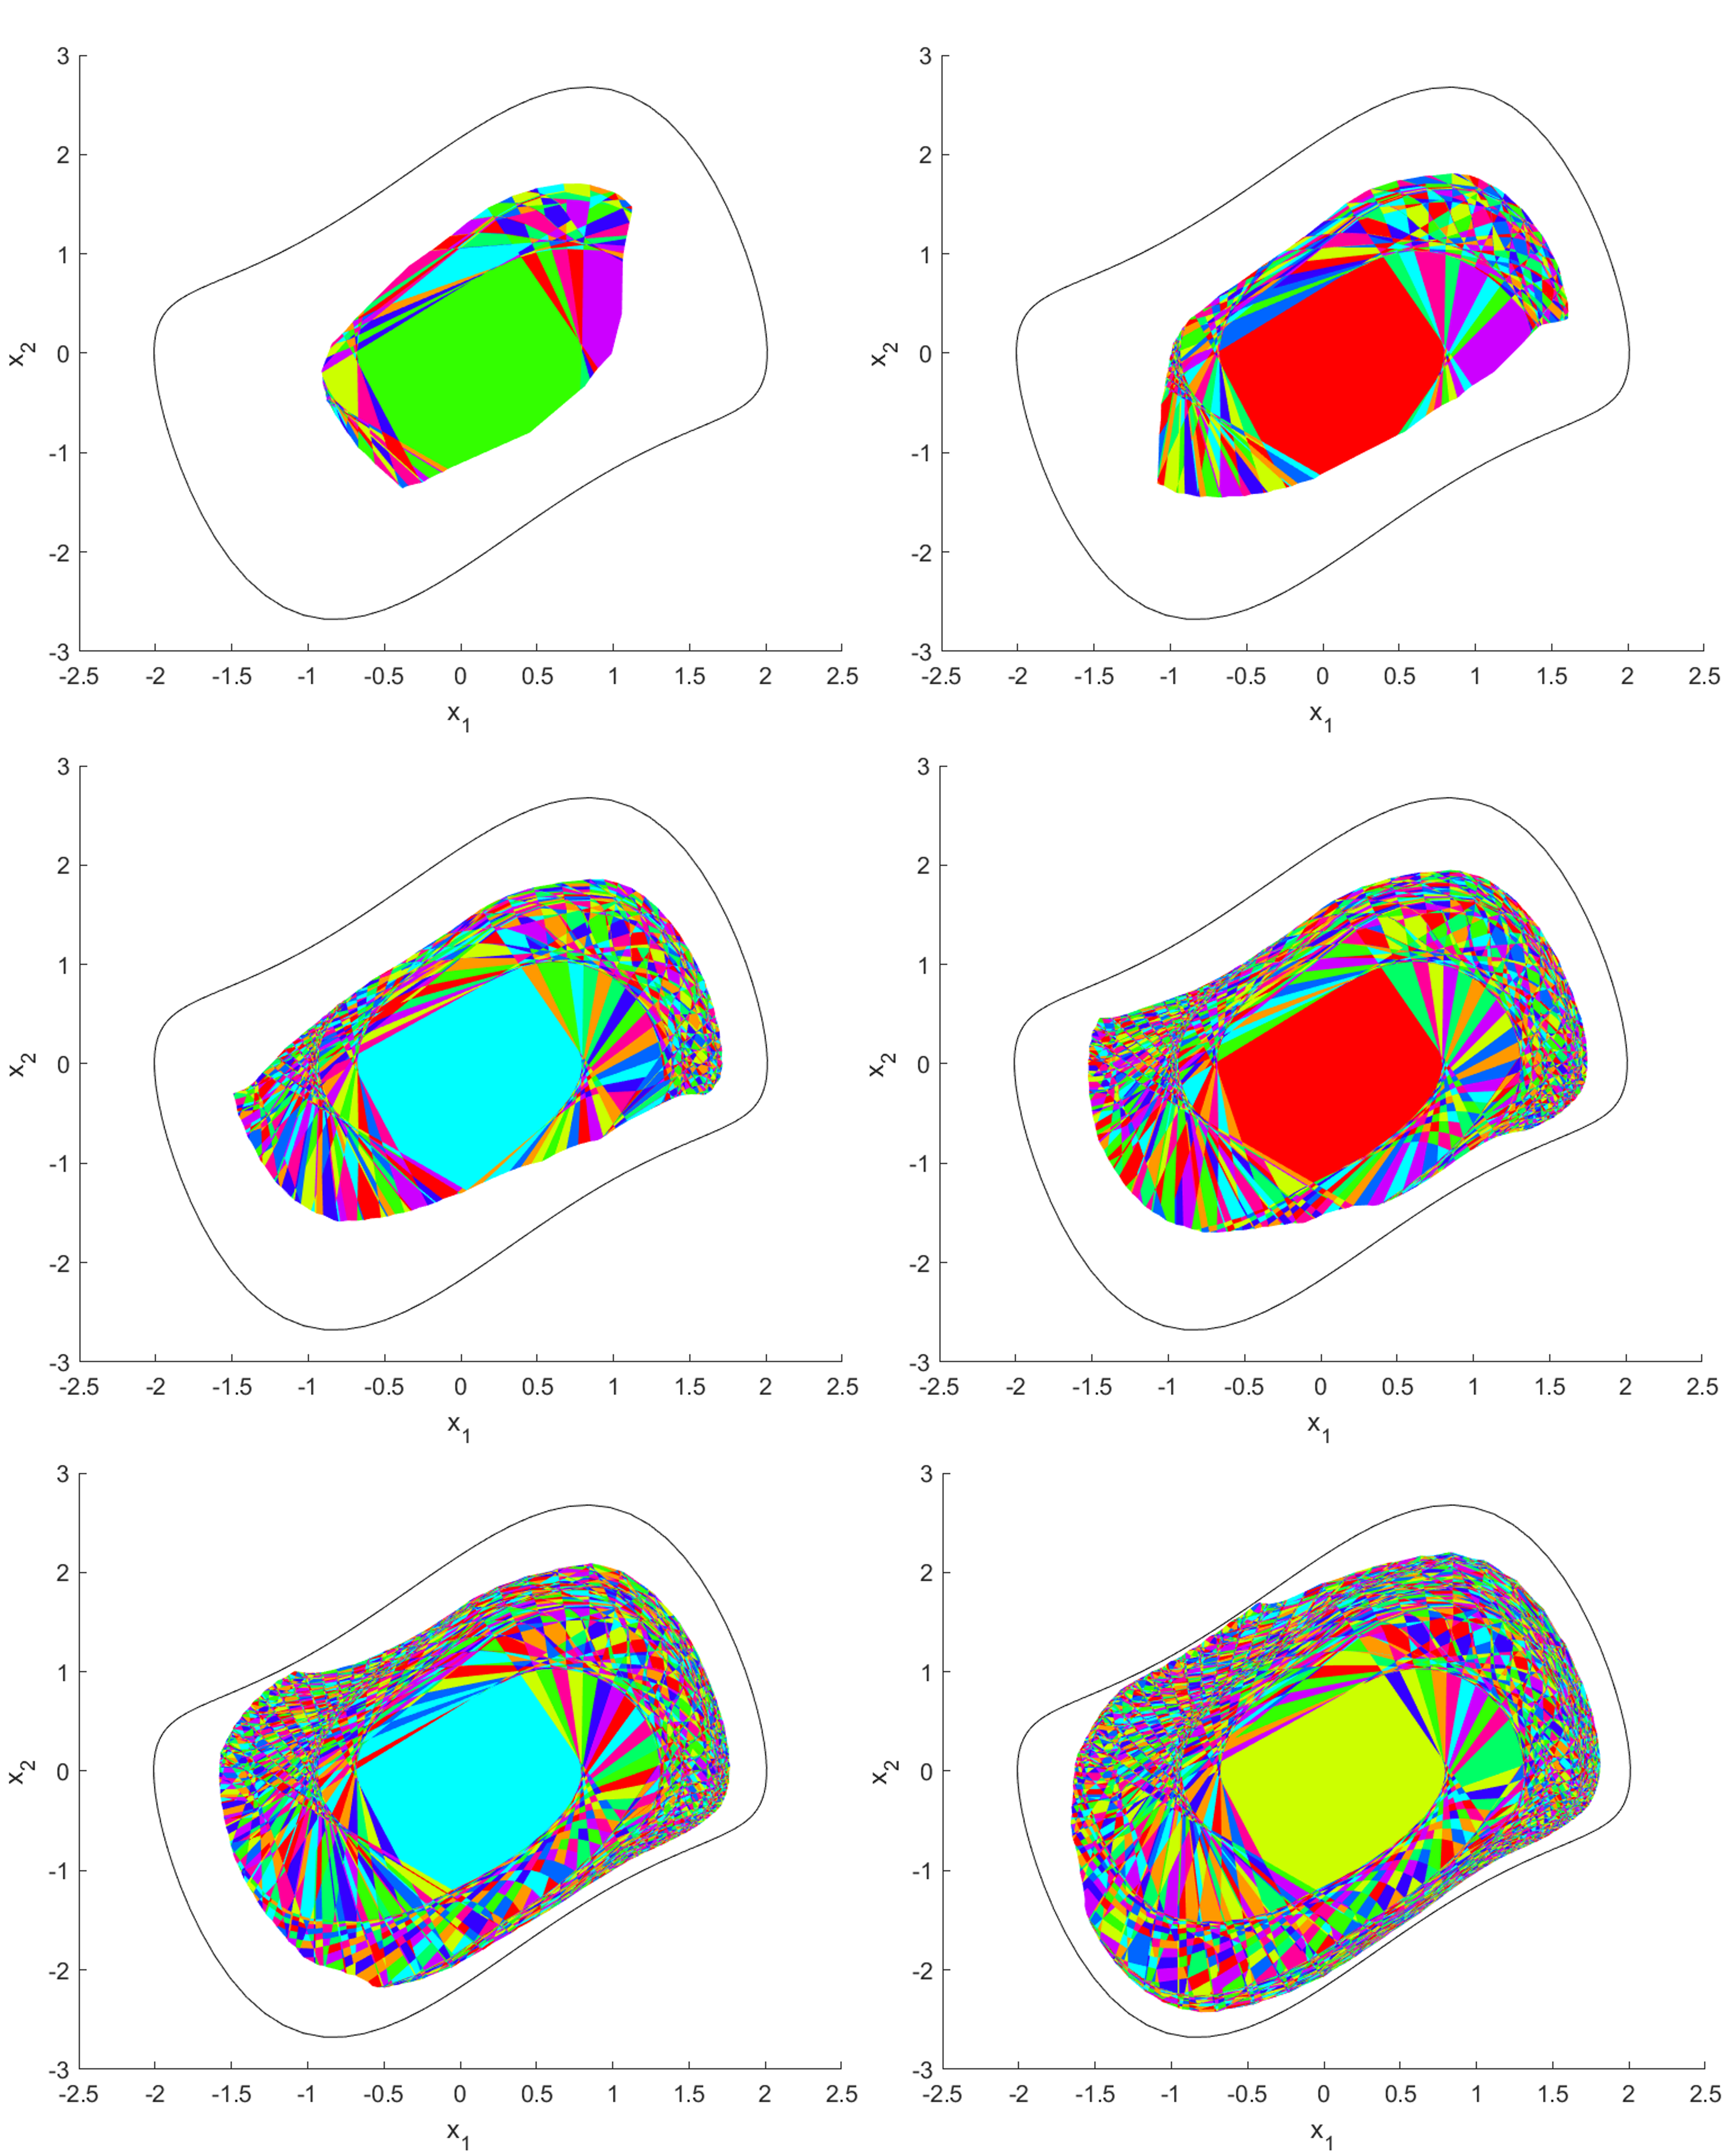
\includegraphics[width=0.98\linewidth]{figs/van_panel_mat.png} 
\setlength\belowcaptionskip{-1.\baselineskip}
\centering
\caption{5, 10, 15, 20, 25, and 30-step regions of attraction (ROAs) for the learned van der Pol system. The learned dynamics network is continuously invertible, implying that preimages of connected sets are connected. This property restricts the space explored with RPM, resulting in a 15x speedup in ROA computation. The black line represents the boundary of the true continuous-time maximal ROA.}
\label{fig:van_panel}
\end{figure}











%%%%%%%%%%%%%%%%%%%%%%%%%%%%%%%%%%%%%%%%%%%%%%%%%%%%%%%%%%%%%%%%%%%%%%%%%%%%%%%%%%%%%
\subsection{Pendulum Example} \label{Pendulum}
In this example we pair our RPM tool with the popular multi-parametric toolbox (MPT3) \cite{MPT3} to find a control invariant set for a learned pendulum model. We first learn a ReLU network that models the continuous-time dynamics
\begin{align}
    \Ddot{\theta} = \frac{u + mgl\sin{\theta}}{ml^2}
\end{align}
as a discrete-time model where $m = 1$kg, $g = 9.81$m/s$^{2}$, $l=1$m, and $\theta$ is measured clockwise from the upright position. 
\textcolor{black}{We repeat the network training and enumeration of affine regions $10$ times and provide ranges for the number of affine regions and computation time in Table \ref{tab:pend_details}.
We run the longer, invariant set computation, on only one of the networks (a network with 217 regions).}

Details of the learned dynamics network are in Table \ref{tab:pend_details}.

% \begingroup
% \setlength{\tabcolsep}{5pt}
% \begin{table}[h]
%     \centering
%     \caption{\textcolor{black}{Pendulum Dynamics Analysis}}
%     {\color{black}\begin{tabular}{c c c}
%         Layer Sizes&\# Affine Regions&Time\\
%         \hline \\ [-1.5ex]
%         $3$, $16$, $16$, $2$ & $217$ & $3$ seconds
%     \end{tabular}}
%     \label{tab:pend_details}
% \end{table} 
% \endgroup

\begingroup
\setlength{\tabcolsep}{5pt}
\begin{table}[h]
    \centering
    \caption{Pendulum Dynamics Analysis}
    {\color{black}\begin{tabular}{c | c}
        Layer Sizes & $3$, $16$, $16$, $2$ \\
        Number of Affine Regions & \textcolor{black}{$217 - 823$} Regions \\
        Time to Enumerate Affine Regions & \textcolor{black}{$2.35 - 4.11$} Seconds
    \end{tabular}}
    \label{tab:pend_details}
\end{table} 
\endgroup




We then use MPT3 to compute the control invariant set shown in Figure \ref{fig:ctrl_inv} with computational details in Table \ref{tab:pend_set}.
% The control invariant set in Figure \ref{fig:ctrl_inv} converged in 61 steps after 5.4 hours of computation, and is represented by 958 polyhedra.

\begingroup
\setlength{\tabcolsep}{5pt}
\begin{table}[h]
    \centering
    \caption{Pendulum Control Invariant Set}
    {\color{black}\begin{tabular}{c c c}
        Algorithm Steps&\# Polyhedra in Set&Time\\
        \hline \\ [-1.5ex]
        $61$ & $958$ & $5.4$ hours
    \end{tabular}}
    \label{tab:pend_set}
\end{table} 
\endgroup

As shown in Figure \ref{fig:ctrl_inv}, the control invariant set is the union of 3 disjoint sets. The leftmost set represents the states for which there is enough control authority to keep the pendulum clockwise of the swing-down position, but not enough to swing back up to upright. The middle set represents the states for which there is enough control authority to keep the pendulum from swinging all the way down. Finally, rightmost set has a similar interpretation to the leftmost set, being the states for which there is enough control authority to keep the pendulum counterclockwise of the swing-down position, but not enough to swing back upright. With the explicit PWA representation given by RPM, the wide array of PWA analysis tools offered by the MPT3 toolbox is able to be leveraged for learned dynamics and controls models.
\begin{figure}[h]
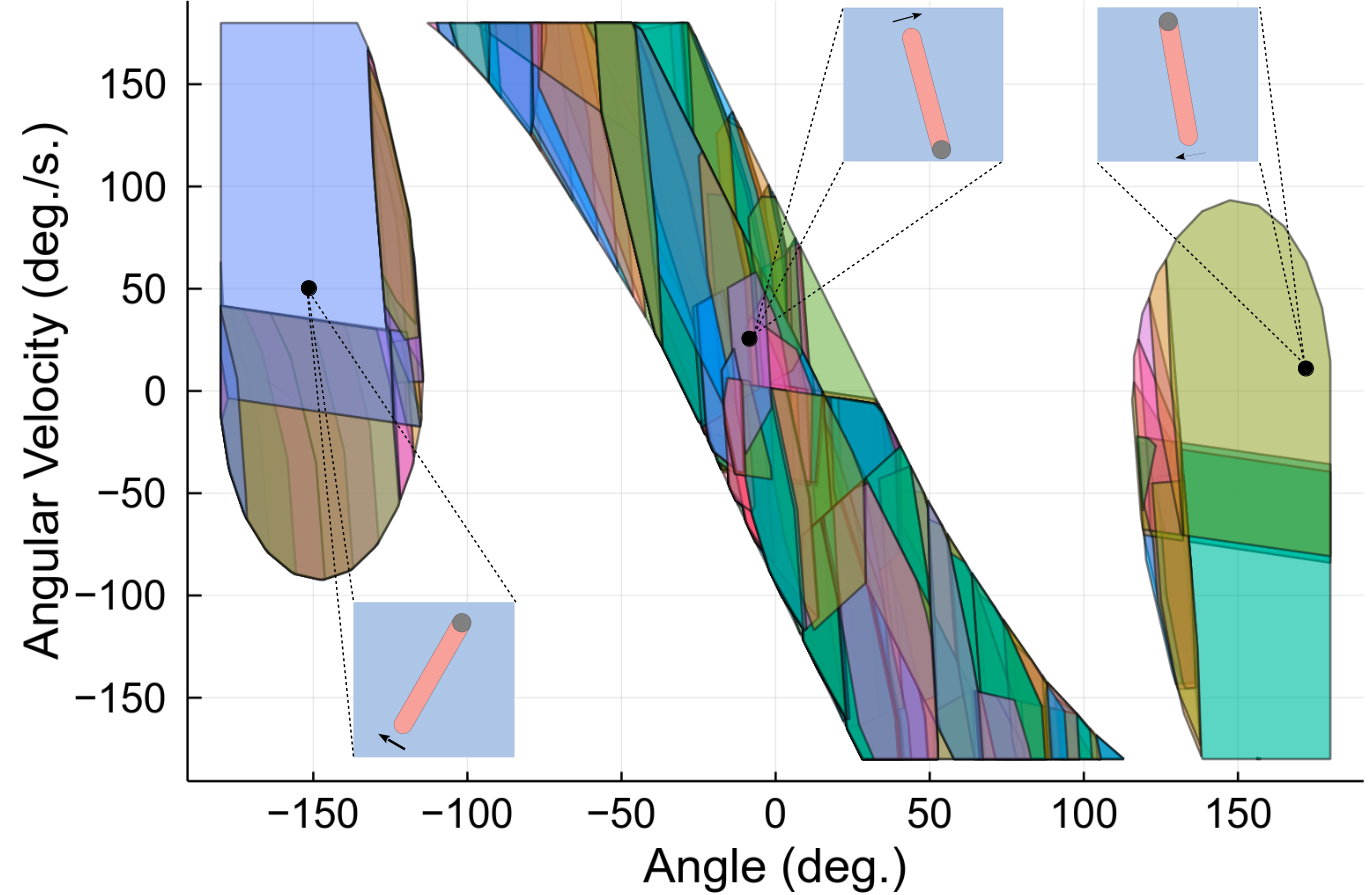
\includegraphics[width=0.85\columnwidth]{figs/ctrl_inv_blowout.png} 
% \setlength\abovecaptionskip{-0.2\baselineskip}
% \setlength\belowcaptionskip{-0.5\baselineskip}
\centering
\caption{A control invariant set for a learned, torque controlled pendulum system. The domain of the dynamics is $\theta \in (-180\degree, 180\degree)$, $\dot{\theta} \in [-180 \degree/\text{s}, 180 \degree/\text{s}]$, $u \in [-5, 5]$ N-m,  where $0\degree$ is upright. Note that we restrict the pendulum so it is not allowed to pass through the down position.  When RPM is paired with MPT3 we are able to compute complicated control invariant sets of learned systems, like this unconnected set, as opposed to convex approximations. Within each connected component a sample state is illustrated to help visualize the possible pendulum configurations.}
\label{fig:ctrl_inv}
\end{figure}

% \begin{figure}
%      \centering
%      \begin{subfigure}[b]{\columnwidth}
%          \centering
%          \includegraphics[width=\textwidth]{figs/ctrl_inv.png}
%          \caption{Control invariant set.}
%          \label{fig:ctrl_inv}
%      \end{subfigure}
%      \hfill
     
%      \begin{subfigure}[b]{0.48\columnwidth}
%          \centering
%          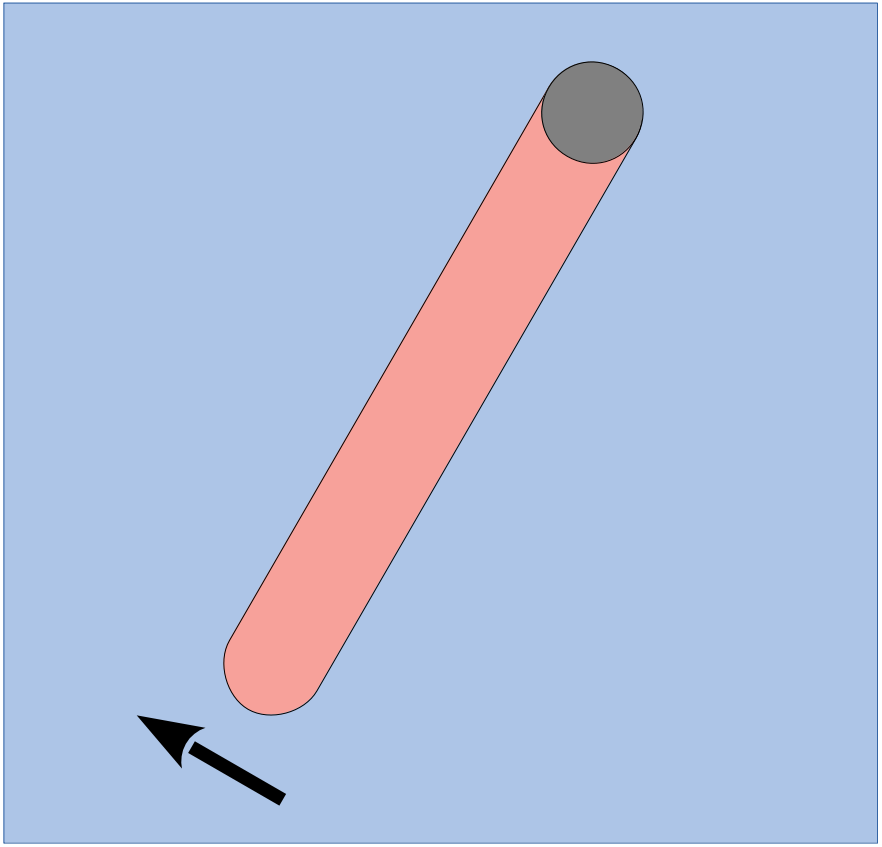
\includegraphics[width=\textwidth]{figs/pend_1.png}
%          \caption{$\theta = -150\degree$, $\dot{\theta} = 50 \degree /$s.}
%          \label{fig:pend_1}
%      \end{subfigure}
%      \hfill
%      \begin{subfigure}[b]{0.48\columnwidth}
%          \centering
%          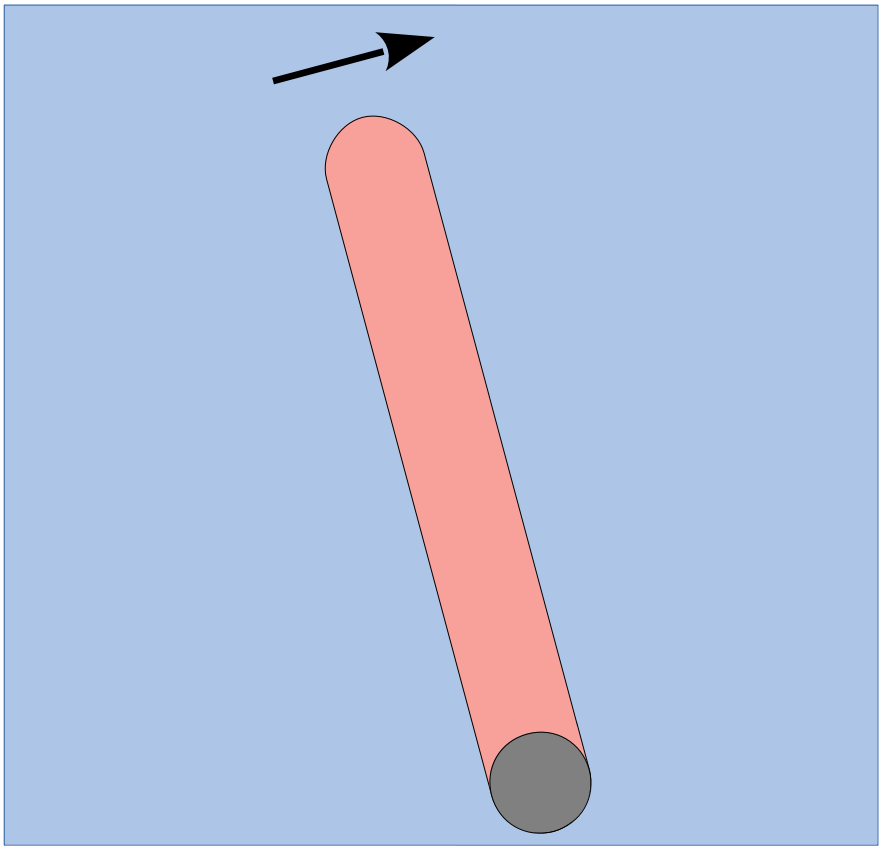
\includegraphics[width=\textwidth]{figs/pend_2.png}
%          \caption{$\theta = -15\degree$, $\dot{\theta} = 25 \degree /$s.}
%          \label{fig:pend_2}
%      \end{subfigure}
%      \hfill
%      \begin{subfigure}[b]{0.48\columnwidth}
%          \centering
%          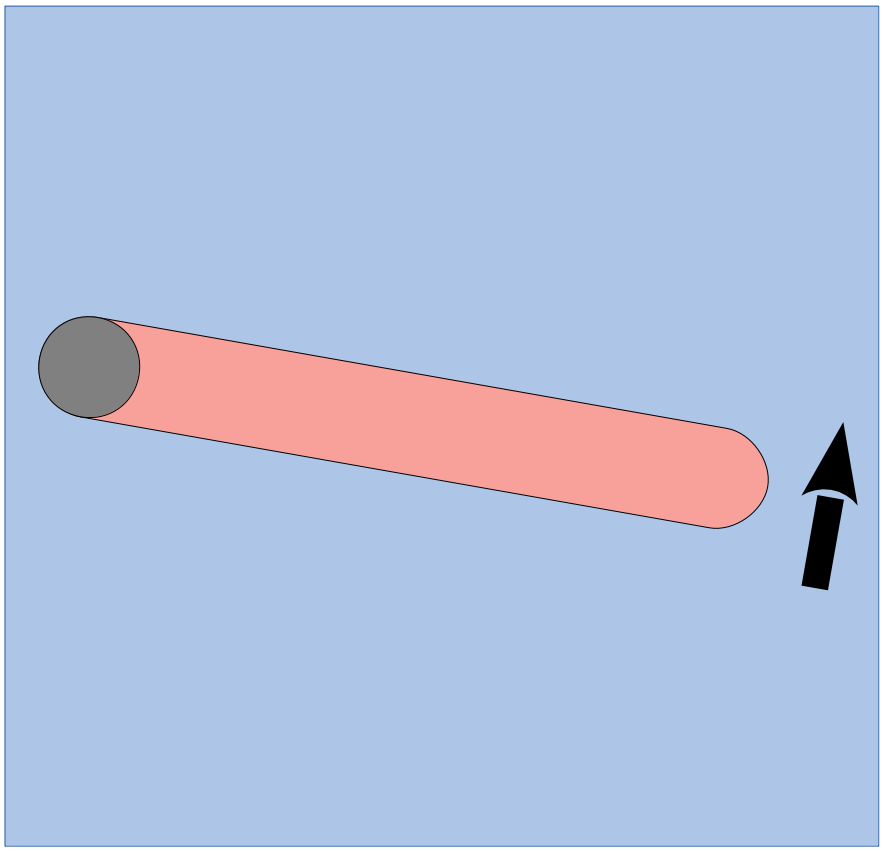
\includegraphics[width=\textwidth]{figs/pend_3.png}
%          \caption{$\theta = 100\degree$, $\dot{\theta} = -170 \degree /$s.}
%          \label{fig:pend_3}
%      \end{subfigure}
%      \hfill
%      \begin{subfigure}[b]{0.48\columnwidth}
%          \centering
%          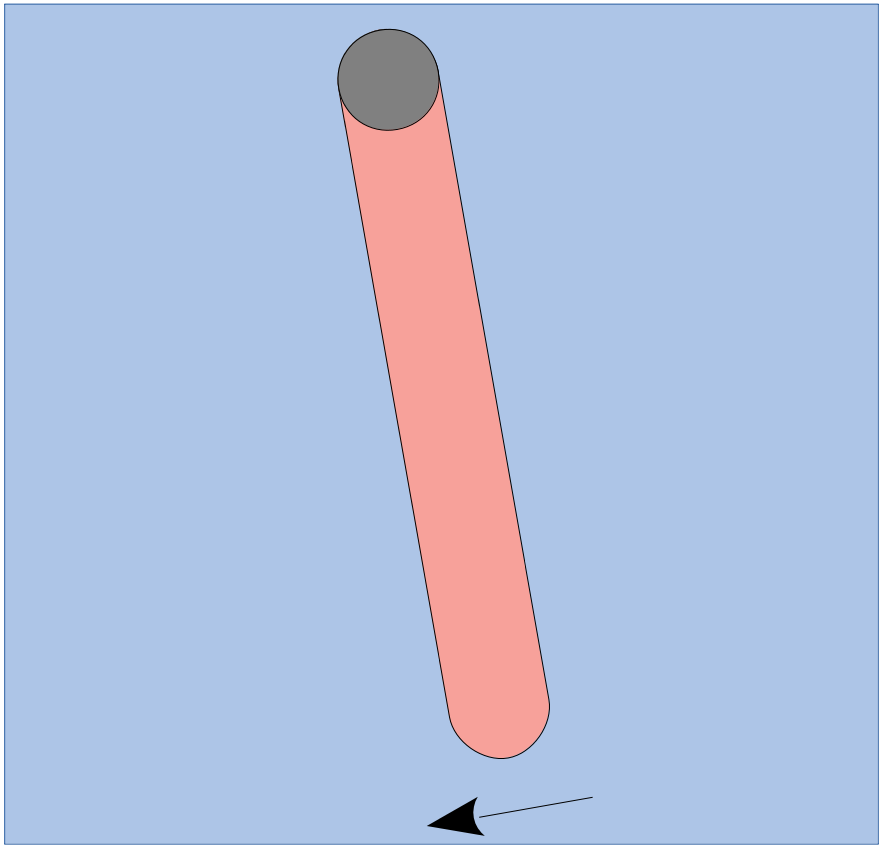
\includegraphics[width=\textwidth]{figs/pend_4.png}
%          \caption{$\theta = 170\degree$, $\dot{\theta} = 10 \degree /$s.}
%          \label{fig:pend_4}
%      \end{subfigure}
%         \caption{A control invariant set (Figure \ref{fig:ctrl_inv}) for a learned, torque controlled pendulum system.  Control invariant set for learned pendulum system with domain $\theta \in [-180\degree, 180\degree]$, $\dot{\theta} \in [-180 \degree/\text{s}, 180 \degree/\text{s}]$, $u \in [-5, 5]$ N-m,  where $0\degree$ is upright.}
%         \label{fig:control_invariant_panel}
% \end{figure}









%%%%%%%%%%%%%%%%%%%%%%%%%%%%%%%%%%%%%%%%%%%%%%%%%%%%%%%
\subsection{Verifying Image-Based Control} \label{Taxinet}
\begin{figure}
    \setlength\abovecaptionskip{1.2\baselineskip}
    \setlength\belowcaptionskip{-0.8\baselineskip}
     \centering
     \begin{subfigure}[b]{0.48\columnwidth}
         \centering
         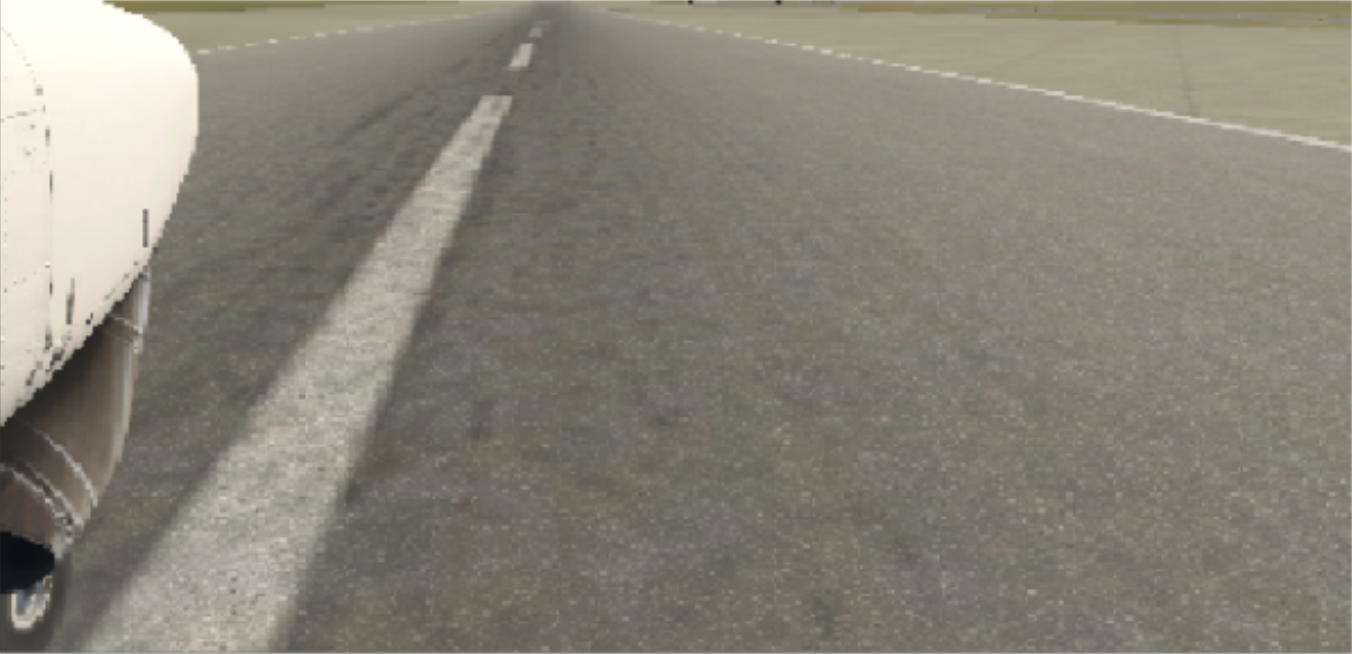
\includegraphics[width=\textwidth]{figs/taxinet_full.png}
         \caption{Full observation.}
         \label{fig:taxinet_full}
     \end{subfigure}
     \hfill
     \begin{subfigure}[b]{0.48\columnwidth}
         \centering
         
\includegraphics[width=\textwidth]{figs/taxinet_coarse.png}
         \caption{Downsampled observation.}
         \label{fig:taxinet_coarse.}
     \end{subfigure}
        \caption{The X-Plane 11 flight simulator is used to generate realistic image observations (left) that are then downsampled (right). The downsampled images are used to learn an image-based controller, as well as to learn an observation model from state to image observation. Putting these two components together along with a learned dynamics network results in closed-loop system dynamics represented as a single ReLU network. These images and learned controller/observation models are from \cite{verify_gan}.}
        \label{fig:taxinet_obs}
\end{figure}

lIn this example we apply the tools of Section \ref{Sec:ROA} to a larger dynamical system that models the closed-loop behavior of a taxiing airplane controlled from camera images.
Our goal is to investigate the set of states that are stabilized by a learned image-based controller by modeling the closed-loop dynamical system with a single ReLU network, and applying the accelerated procedure from Section \ref{Sec:ROA}. 

The specific system we consider was introduced in \cite{verify_gan} where a taxiing airplane is regulated to the centerline of a runway via rudder-angle control input based on images from an onboard camera. Because of the image observation, we cannot model the observation from physical principles. Instead, we modify the learned models in \cite{verify_gan} to obtain a network that approximates the observed image given a state
\begin{align}
    \mathbf{o}_t = F_{obs}(\bx_t),
\end{align}
and a control network that produces a rudder angle command given an observed image
\begin{align}
    u = F_{ctrl}(\mathbf{o}_t).
\end{align}
The continuous time dynamics are
\begin{subequations}
\begin{align}
    \dot{p} &= v\sin{\theta} \\
    \dot{\theta} &= \frac{v}{L}\tan{u}
\end{align}
\end{subequations}
for crosstrack position $p$, heading error $\theta$, rudder angle $u$, and speed $v=5$ m/s. We learn a 1Hz discrete-time model,
\begin{align}
    \bx_{t+1} = F_{dyn}(\bx_t, u),
\end{align}
and then have the closed-loop system
\begin{align}
    \bx_{t+1} = F_{cl}(\bx_t) = F_{dyn}(\bx_t, F_{ctrl} \circ F_{obs}(\bx_t))
\end{align}
which can be represented as one ReLU network.

Next, we use Algorithm \ref{Algo:cell_enumeration} to retrieve the explicit PWA function for $F_{cl}$ over the domain $p \in [-5, 5]$ m., $\theta \in [-15^\circ, 15^\circ]$. 
The resulting PWA function has 244,920 regions, took 3 hours to compute, and was not found to be a homeomorphism.
Timing for these steps is summarized in Table \ref{tab:taxinet_details}.
Although the function is not homeomorphic, when applying the accelerated algorithm from Section \ref{sec:homeo}, we are still guaranteed that all states within this set asymptotically converge to the stable fixed point.


% \begingroup
% \setlength{\tabcolsep}{5pt}
% \begin{table}[h]
%     \centering
%     \caption{\textcolor{black}{Image-Based Control Dynamics Analysis}}
%     {\color{black}\begin{tabular}{c c c}
%         Layer Sizes&\# Affine Regions&Time\\
%         \hline \\ [-1.5ex]
%         $2$, $260$, $260$, $260$, $260$, $20$, $12$, $12$, $16$, $2$ & $244,920$ & $3$ hours
%     \end{tabular}}
%     \label{tab:taxinet_details}
% \end{table} 
% \endgroup

\begingroup
\setlength{\tabcolsep}{5pt}
\begin{table}[h]
    \centering
    \caption{Image-Based Control Dynamics Analysis}
    {\color{black}\begin{tabular}{c | c}
        Layer Sizes & \begin{tabular}{@{}c@{}}$2$, $260$, $260$, $260$, $260$, \\ $20$, $12$, $12$, $16$, $2$\end{tabular} 
          \\
        Number of Affine Regions & $244,920$ Regions \\
        Time to Enumerate Affine Regions & $3$ Hours \\
        Time to Check if Homeomorphism & $0.04$ Seconds \\
        Time to Find Fixed Point & $2$ Seconds \\
        Time to Find Seed ROA & $3$ Seconds
    \end{tabular}}
    \label{tab:taxinet_details}
\end{table} 
\endgroup

This PWA function is significantly larger than other PWA dynamics that have been studied in the literature ($\sim 250,000$ regions vs $\sim 1,000$ regions). 
After computing the explicit PWA function, we find a stable fixed point. Next, we find a seed ROA for each stable fixed point and perform backward reachability to grow the ROAs. During the backward reachability computation, we use a few strategies to make the problem more tractable. First, we restrict the backward reachability algorithm to only explore connected backward reachable sets as described in Section \ref{sec:homeo}. 
Second, to avoid numerical concerns accompanied with very small polyhedra, we compute backward reachable sets iteratively with the 1-step PWA dynamics directly instead of in one shot using concatenated ReLU networks. 
Third, at each step we merge the polyhedra into a union of overlapping polyhedra to reduce the complexity of the set representation.

In Figure \ref{fig:taxi_roa} we show the set of states that our algorithm was able to show is asymptotically stabilized by the learned controller.
This set was computed using $11$ backward reachable steps (11 seconds of trajectory evolution), and is represented as a union of $28,715$ polyhedra.


\begingroup
\setlength{\tabcolsep}{5pt}
\begin{table}[h]
    \centering
    \caption{Image-Based Control ROA}
    {\color{black}\begin{tabular}{c c c}
        Algorithm Steps&\# Polyhedra in Set&Time\\
        \hline \\ [-1.5ex]
        $11$ & $28,715$ & $14$ hours
    \end{tabular}}
    \label{tab:taxinet_roa}
\end{table} 
\endgroup

\begin{figure}
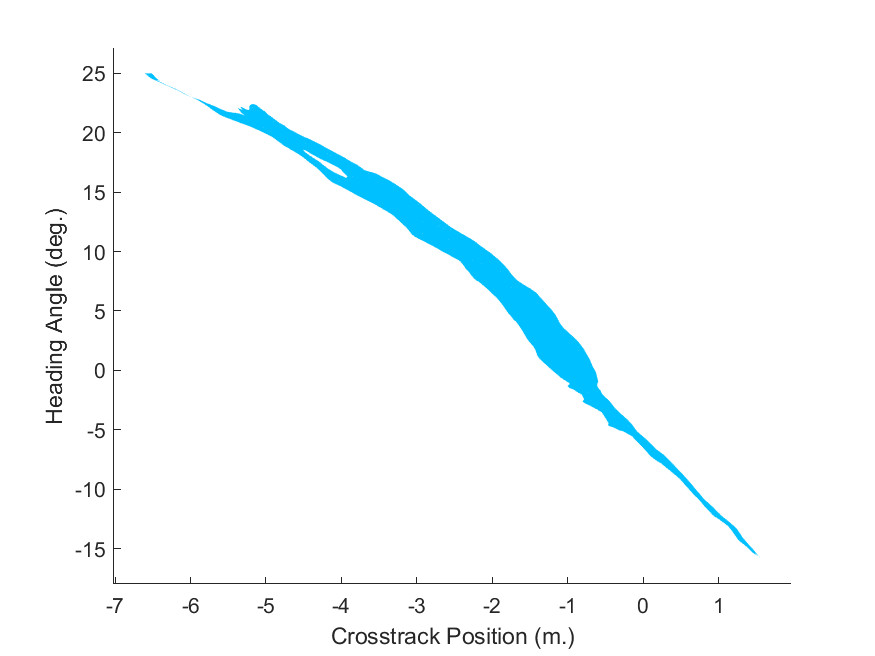
\includegraphics[width = 0.85\linewidth]{figs/taxinet_11.png} 
% \setlength\abovecaptionskip{-0.1\baselineskip}
\setlength\belowcaptionskip{-1.\baselineskip}
\centering
\caption{Set of states that our approach finds are stabilized by the learned controller for the image-based airplane runway taxiing system from Fig.~\ref{fig:taxinet_obs}.
This set is the 11-step backward reachable set for the seed ROA found around the stable fixed point.
This set of states is represented by 28,715 polyhedra.
}
\label{fig:taxi_roa}
\end{figure}